%%%%%%%%%%%%%%%%%%%%%%%%%%%%%%%%%%%%%%%%%
% Beamer Presentation
% LaTeX Template
% Version 1.0 (10/11/12)
%
% This template has been downloaded from:
% http://www.LaTeXTemplates.com
%
% License:
% CC BY-NC-SA 3.0 (http://creativecommons.org/licenses/by-nc-sa/3.0/)
%
%%%%%%%%%%%%%%%%%%%%%%%%%%%%%%%%%%%%%%%%%

%----------------------------------------------------------------------------------------
%	PACKAGES AND THEMES
%----------------------------------------------------------------------------------------

% \documentclass{beamer}
\documentclass[handout]{beamer}


\mode<presentation> {

\usetheme{Madrid}

}

\definecolor{DataBlue}{rgb}{0.50, 0.85, 0.99} 

\setbeamercolor{titlelike}{parent=structure,bg=black, fg = white}
\setbeamercolor{frametitle}{fg=white}
\usepackage{graphicx} % Allows including images
\usepackage{booktabs} % Allows the use of \toprule, \midrule and \bottomrule in tables
\usepackage[export]{adjustbox}
\usepackage[portuguese]{babel}
\usepackage[utf8]{inputenc}

\usepackage{pgfplots}
\usepackage{tikz}
\usetikzlibrary{calc,babel,quotes,angles}
\usepackage{tkz-euclide}

\usepackage{amsmath, amsfonts, amssymb}

\usepackage{cancel}

\usepackage{multirow}
% \usepackage{xcolor}

\makeatletter
\let\save@measuring@true\measuring@true
\def\measuring@true{%
  \save@measuring@true
  \def\beamer@sortzero##1{\beamer@ifnextcharospec{\beamer@sortzeroread{##1}}{}}%
  \def\beamer@sortzeroread##1<##2>{}%
  \def\beamer@finalnospec{}%
}
\makeatother


%----------------------------------------------------------------------------------------
%	TITLE PAGE
%----------------------------------------------------------------------------------------

\title{Geometria} %% Title
\subtitle{Aula 03}
\author{Gustavo Ale} % Your name
\institute[UFMT] % Your institution as it will appear on the bottom of every slide, may be shorthand to save space
{
EduCursinho - Faculdade de Engenharia \\ % Your institution for the title page
\medskip
\textit{gustavo.engca@gmail.com} % Your email address
}
\date{\today} % Date, can be changed to a custom date

% Rodapé
% \setbeamertemplate{footline}{%
%     \begin{beamercolorbox}[wd=\paperwidth]{footlinecolor}
%         \includegraphics[width=\paperwidth]{images/footbar.png}
%     \end{beamercolorbox}%
% }

\begin{document}
{
\setbeamertemplate{footline}{}
\begin{frame}
    \begin{columns}
        \begin{column}{0.48\textwidth}
            % \hspace*{-1cm}
            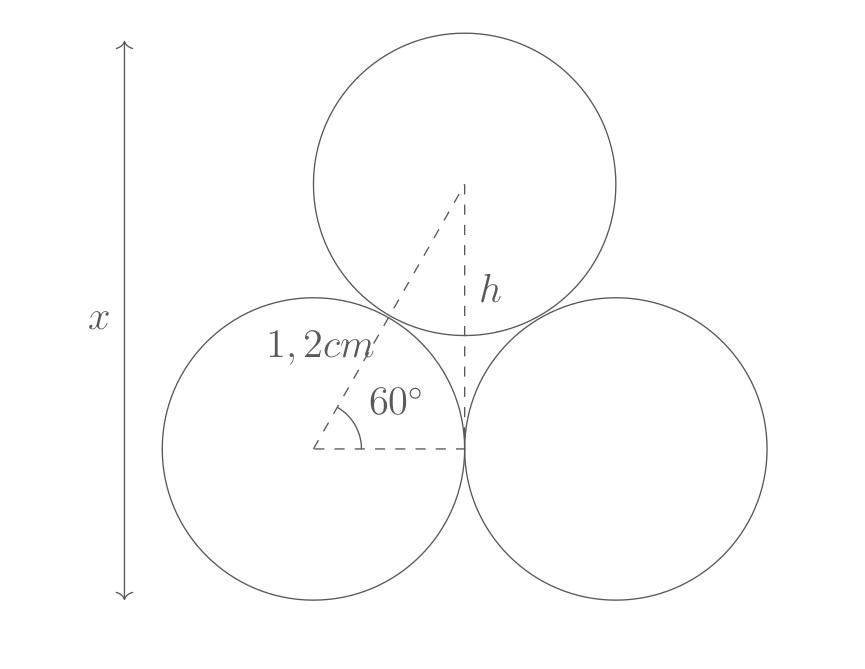
\includegraphics[width=\columnwidth,left]{../assets/geo.png}
        \end{column}
        \begin{column}{0.48\textwidth}
            \titlepage
        \end{column}
    \end{columns}

\end{frame}
}

%-------------------------------------------------------------------------------
% Sumário
%-------------------------------------------------------------------------------

\begin{frame}
    \frametitle{Sumário} % Table of contents slide, comment this block out to remove it
    \tableofcontents % Throughout your presentation, if you choose to use \section{} and \subsection{} commands, these will automatically be printed on this slide as an overview of your presentation
\end{frame}

%----------------------------------------------------------------------------------------
%	PRESENTATION SLIDES
%----------------------------------------------------------------------------------------

\section{Funções trigonométricas}
\subsection{Nomenclaturas}
\begin{frame}[fragile]\frametitle{\subsecname}
    Dado o triângulo retângulo $ABC$ abaixo:
    \begin{figure}[H]
        \centering
        %\resizebox{\columnwidth}{!}{%
        \begin{tikzpicture}[scale=0.7\columnwidth/10cm]
            \coordinate (A) at (0,0);
            \coordinate (B) at (4,3);
            \coordinate (C) at (4,0);
            % \coordinate (D) at (0,3);
            \node[circle, fill, label={left:$A$}, inner sep=2pt] at (A) {};
            \node[circle, fill, label={right:$B$}, inner sep=2pt] at (B) {};
            \node[circle, fill, label={right:$C$}, inner sep=2pt] at (C) {};
            % \node[circle, fill, label={left:$D$}, inner sep=2pt] at (D) {};
            % \draw[dashed] (A)--(D)--(B);
            \draw (A)-- node[above left] {$hip$} (B);
            \draw (B)-- node[right] {$CO$} (C);
            \draw (C)-- node[below] {$CA$} (A);
            \pic ["$\theta$", draw, -,angle eccentricity=2] {angle = C--A--B};
            \tkzMarkRightAngle[size=.3](A,C,B);
        \end{tikzpicture}
        %}
        % \caption{Triângulo retângulo $ABC$}
    \end{figure}
    \noindent A aresta $\overline{AB}$ é denominada hipotenusa ou abreviadamente $hip$,
    a aresta $\overline{BC}$ é denominada cateto oposto ou $CO$ e a aresta
    $\overline{AC}$ é denominada cateto adjacente ou $CA$
\end{frame}

\begin{frame}[fragile]\frametitle{\subsecname}
    \begin{figure}[H]
        \centering
        %\resizebox{\columnwidth}{!}{%
        \begin{tikzpicture}[scale=0.7\columnwidth/10cm]
            \coordinate (A) at (0,0);
            \coordinate (B) at (4,3);
            \coordinate (C) at (4,0);
            % \coordinate (D) at (0,3);
            \pic ["$\theta$", draw, -,angle eccentricity=2] {angle = A--B--C};
            \node[circle, fill, label={left:$A$}, inner sep=2pt] at (A) {};
            \node[circle, fill, label={right:$B$}, inner sep=2pt] at (B) {};
            \node[circle, fill, label={right:$C$}, inner sep=2pt] at (C) {};
            % \node[circle, fill, label={left:$D$}, inner sep=2pt] at (D) {};
            % \draw[dashed] (A)--(D)--(B);
            \tkzMarkRightAngle[size=.3](A,C,B);
            \draw (B)-- (C);
            \draw (C)-- (A);
            \draw (A)-- (B); \pause
            \draw (B)-- node[right] {$CA$} (C); \pause
            \draw (C)-- node[below] {$CO$} (A); \pause
            \draw (A)-- node[above left] {$hip$} (B);
        \end{tikzpicture}
        %}
        % \caption{Triângulo retângulo $ABC$}
    \end{figure}

\end{frame}

%------------------------------------------------

\subsection{Relação com o triângulo retângulo}
\begin{frame}\frametitle{\subsecname}
    
    \begin{align}
        sen(\theta) & = \frac{CO}{hip} \\[1ex]
        cos(\theta) & = \frac{CA}{hip} \\[1ex]
        tg(\theta)  & = \frac{CO}{CA}
    \end{align}

\end{frame}

%------------------------------------------------

\subsection{Valores das funções trigonométricas}
\begin{frame}\frametitle{\subsecname}

    Devido a complexidade em se cálcular o resultado das funções trigonométricas
    seno, cosseno e tangente, muitos exercícios que envolvem essas funções acabam
    por usar valores bem conhecidos, ou valores tabelados, isso é verdade
    principalmente para os vestibulares.
    
\end{frame}

\begin{frame}\frametitle{\subsecname}

    \begin{table}[H]
        % \setlength\extrarowheight{1cm}
        \renewcommand\arraystretch{2.5}
        % \newcolumntype{C}{>{$\displaystyle}c<{$}}
        \centering
        \resizebox{0.6\textwidth}{!}{%
            \begin{tabular}{c|c|c|c}
                    & 30° $\displaystyle \left(\frac{\pi}{6}\right)$                      & 45° $\displaystyle \left(\frac{\pi}{4}\right)$                      & 60° $\displaystyle \left(\frac{\pi}{3}\right)$                       \\ \hline
                sen & $\displaystyle \frac{1}{2}$        & $\displaystyle \frac{\sqrt{2}}{2}$ & $\displaystyle \frac{\sqrt{3}}{2}$ \\ \hline
                cos & $\displaystyle \frac{\sqrt{3}}{2}$ & $\displaystyle \frac{\sqrt{2}}{2}$ & $\displaystyle \frac{1}{2}$        \\ \hline
                tg  & $\displaystyle \frac{\sqrt{3}}{3}$ & $1$                                & $\sqrt{3}$
            \end{tabular}%
        }
        \caption{Tabela seno, cosseno e tangente}
        \label{tab:trig_val}
    \end{table}

\end{frame}

%------------------------------------------------


%------------------------------------------------

\subsection{Exercícios}


\begin{frame}[fragile]\frametitle{\subsecname}
    Encontre o valor de $x$ para as seguintes fíguras:
\begin{columns}
    \column{0.5\textwidth}
        a)
        \begin{figure}[H]
            \centering
            %\resizebox{\columnwidth}{!}{%
            \begin{tikzpicture}[scale=\textwidth/10cm]
                \coordinate (A) at (0,0);
                \coordinate (B) at (4,3);
                \coordinate (C) at (4,0);
                % \coordinate (D) at (0,3);
                \pic ["$45^\circ$", draw, -,angle eccentricity=2] {angle = A--B--C};
                % \node[circle, fill, label={left:$A$}, inner sep=2pt] at (A) {};
                % \node[circle, fill, label={right:$B$}, inner sep=2pt] at (B) {};
                % \node[circle, fill, label={right:$C$}, inner sep=2pt] at (C) {};
                % \node[circle, fill, label={left:$D$}, inner sep=2pt] at (D) {};
                % \draw[dashed] (A)--(D)--(B);
                \tkzMarkRightAngle[size=.3](A,C,B);
                \draw (B)-- (C);
                \draw (C)-- (A);
                \draw (A)-- (B);
                % \draw (B)-- node[right] {$CA$} (C); 
                \draw (C)-- node[below] {$x$} (A); 
                \draw (A)-- node[above left] {$4$} (B);
            \end{tikzpicture}
            %}
            % \caption{Triângulo retângulo $ABC$}
        \end{figure}

        \column{0.5\textwidth}
        b)
        \begin{figure}[H]
            \centering
            %\resizebox{\columnwidth}{!}{%
            \begin{tikzpicture}[scale=\columnwidth/10cm]
                \coordinate (A) at (0,0);
                \coordinate (B) at (4,3);
                \coordinate (C) at (4,0);
                % \coordinate (D) at (0,3);
                \pic ["$30^\circ$", draw, -,angle eccentricity=2] {angle = C--A--B};
                % \node[circle, fill, label={left:$A$}, inner sep=2pt] at (A) {};
                % \node[circle, fill, label={right:$B$}, inner sep=2pt] at (B) {};
                % \node[circle, fill, label={right:$C$}, inner sep=2pt] at (C) {};
                % \node[circle, fill, label={left:$D$}, inner sep=2pt] at (D) {};
                % \draw[dashed] (A)--(D)--(B);
                \tkzMarkRightAngle[size=.3](A,C,B);
                \draw (B)-- (C);
                \draw (C)-- (A);
                \draw (A)-- (B);
                \draw (B)-- node[right] {$x$} (C); 
                \draw (C)-- node[below] {$5$} (A); 
                % \draw (A)-- node[above left] {$4$} (B);
            \end{tikzpicture}
            %}
            % \caption{Triângulo retângulo $ABC$}
        \end{figure}

\end{columns}

\end{frame}


%------------------------------------------------

\begin{frame}
    \Huge{\centerline{Perguntas?}}
\end{frame}

%----------------------------------------------------------------------------------------

\end{document}